%%
%% This is file `sample-acmlarge.tex',
%% generated with the docstrip utility.
%%
%% The original source files were:
%%
%% samples.dtx  (with options: `all,journal,bibtex,acmlarge')
%% 
%% IMPORTANT NOTICE:
%% 
%% For the copyright see the source file.
%% 
%% Any modified versions of this file must be renamed
%% with new filenames distinct from sample-acmlarge.tex.
%% 
%% For distribution of the original source see the terms
%% for copying and modification in the file samples.dtx.
%% 
%% This generated file may be distributed as long as the
%% original source files, as listed above, are part of the
%% same distribution. (The sources need not necessarily be
%% in the same archive or directory.)
%%
%%
%% Commands for TeXCount
%TC:macro \cite [option:text,text]
%TC:macro \citep [option:text,text]
%TC:macro \citet [option:text,text]
%TC:envir table 0 1
%TC:envir table* 0 1
%TC:envir tabular [ignore] word
%TC:envir displaymath 0 word
%TC:envir math 0 word
%TC:envir comment 0 0
%%
%% The first command in your LaTeX source must be the \documentclass
%% command.
%%
%% For submission and review of your manuscript please change the
%% command to \documentclass[manuscript, screen, review]{acmart}.
%%
%% When submitting camera ready or to TAPS, please change the command
%% to \documentclass[sigconf]{acmart} or whichever template is required
%% for your publication.
%%
%%
\documentclass[acmlarge]{acmart}
%%
%% \BibTeX command to typeset BibTeX logo in the docs
\AtBeginDocument{%
  \providecommand\BibTeX{{%
    Bib\TeX}}}

%% Rights management information.  This information is sent to you
%% when you complete the rights form.  These commands have SAMPLE
%% values in them; it is your responsibility as an author to replace
%% the commands and values with those provided to you when you
%% complete the rights form.
\setcopyright{acmlicensed}
\copyrightyear{2018}
\acmYear{2018}
\acmDOI{XXXXXXX.XXXXXXX}

%%
%% These commands are for a JOURNAL article.
\acmJournal{POMACS}
\acmVolume{37}
\acmNumber{4}
\acmArticle{111}
\acmMonth{8}

%%
%% Submission ID.
%% Use this when submitting an article to a sponsored event. You'll
%% receive a unique submission ID from the organizers
%% of the event, and this ID should be used as the parameter to this command.
%%\acmSubmissionID{123-A56-BU3}

%%
%% For managing citations, it is recommended to use bibliography
%% files in BibTeX format.
%%
%% You can then either use BibTeX with the ACM-Reference-Format style,
%% or BibLaTeX with the acmnumeric or acmauthoryear sytles, that include
%% support for advanced citation of software artefact from the
%% biblatex-software package, also separately available on CTAN.
%%
%% Look at the sample-*-biblatex.tex files for templates showcasing
%% the biblatex styles.
%%

%%
%% The majority of ACM publications use numbered citations and
%% references.  The command \citestyle{authoryear} switches to the
%% "author year" style.
%%
%% If you are preparing content for an event
%% sponsored by ACM SIGGRAPH, you must use the "author year" style of
%% citations and references.
%% Uncommenting
%% the next command will enable that style.
%%\citestyle{acmauthoryear}

\usepackage{afterpage}
\usepackage{booktabs} % For formal tables
\usepackage{tabularx}
\usepackage[ruled,linesnumbered]{algorithm2e} % For algorithms
\usepackage{algpseudocode} % For algorithmic environment
\usepackage{array}
\usepackage{rotating}
\usepackage{longtable}
\usepackage{graphicx}
\graphicspath{{figures/}{paper/figures/}}
\usepackage{wrapfig}
\usepackage[T1]{fontenc}
\usepackage[scaled=0.75]{beramono}
\usepackage{listings}
\lstset{language=SQL,morekeywords={PREFIX, java,rdf,rdfs,url}}
\usepackage{tcolorbox}
\usepackage{float}
\usepackage{colortbl}
\definecolor{customgray}{HTML}{ABABAB}
\usepackage{placeins}
\usepackage{adjustbox}
\usepackage{multirow}
\usepackage[para]{footmisc}
\usepackage{threeparttable}
\usepackage{makecell}
\usepackage{lscape}
\usepackage[utf8]{inputenc}
\usepackage{pifont}
\usepackage{newunicodechar}
\newunicodechar{✓}{\ding{51}}
\newunicodechar{✗}{\ding{55}}
\usepackage{xcolor,colortbl}
\usepackage{svg} % For SVG graphics
\usepackage{subcaption}
\setlength{\intextsep}{3pt}  
\setlength{\textfloatsep}{1pt}
\setlength{\abovecaptionskip}{0pt}
\setlength{\belowcaptionskip}{0pt}
% \usepackage{caption} % Do not load: acmart manages captions
% \usepackage{xcolor} % already loaded above with colortbl

%%
%% end of the preamble, start of the body of the document source.
\begin{document}

%%
%% The "title" command has an optional parameter,
%% allowing the author to define a "short title" to be used in page headers.
\title[OntoSage: Easy-Deploy Conversational AI for Sustainable Smart Buildings]{OntoSage: Easy-Deploy Conversational AI for Sustainable Smart Buildings}
\subtitle{Enabling Zero-Knowledge Human-Building Interaction for persona agnostic multi-objective goals}

%%
%% The "author" command and its associated commands are used to define
%% the authors and their affiliations.
%% Of note is the shared affiliation of the first two authors, and the
%% "authornote" and "authornotemark" commands
%% used to denote shared contribution to the research.
\author{Suhas Devmane}
% \authornote{Both authors contributed equally to this research.}
% \email{trovato@corporation.com}
\orcid{1234-5678-9012-3456}
\authornotemark[1]
\email{DevmaneSP1@cardiff.ac.uk}
\affiliation{%
  \institution{Cardiff University}
  \city{Cardiff}
  \state{wALES}
  \country{UK}
}

\author{Omer Rana}
\affiliation{%
  \institution{Cardiff University}
  \country{UK}}
\email{RanaOF@cardiff.ac.uk}

\author{Charith Perera}
\affiliation{%
  \institution{Cardiff University}
  \country{UK}}
\email{PereraC@cardiff.ac.uk}

%%
%% By default, the full list of authors will be used in the page
%% headers. Often, this list is too long, and will overlap
%% other information printed in the page headers. This command allows
%% the author to define a more concise list
%% of authors' names for this purpose.
\renewcommand{\shortauthors}{Devmane et al.}

%%
%% The abstract is a short summary of the work to be presented in the
%% article.

% Abstract
\begin{abstract}
The proliferation of smart building technologies has generated vast sensor data, yet complex building management systems (BMS) create significant barriers to effective Human-Building Interaction (HBI). Traditional interfaces require specialized knowledge of sensor taxonomies and query languages, preventing diverse stakeholders—from facility managers to occupants—from leveraging data for sustainability goals aligned with standards such as LEED, BREEAM, and ASHRAE.

This paper presents OntoSage, a semantic conversational AI framework designed to democratize building data access through natural language question answering. OntoSage integrates BrickSchema ontologies for semantic knowledge representation, GraphDB-based Retrieval-Augmented Generation (RAG) for SPARQL translation, modular analytics agents for sustainability applications, and LangGraph-orchestrated LLM workflows to enable zero-knowledge interaction across heterogeneous building environments. We evaluated OntoSage through a two-phase study: surveying 42 diverse stakeholders to collect authentic information needs, then systematically testing across 10 heterogeneous building environments including one real-world academic testbed (680 sensors, MySQL) and nine synthetic configurations with varying databases (PostgreSQL, TimescaleDB, Cassandra). Results demonstrate high question-answering accuracy with a mean System Usability Scale score of 78.4/100. OntoSage achieved 87.3\% task completion rate, reducing information retrieval time by 66.4\% compared to traditional methods, while enabling rapid cross-building adaptation with 90\% reduction in development effort (28-40 person-hours per building). This work provides empirical validation that semantic AI can effectively bridge the gap between complex building telemetry and actionable sustainability insights for non-expert users.
\end{abstract}

% CCS Concepts (placeholder)
% Replace with appropriate ACM CCS concepts
\begin{CCSXML}
\end{CCSXML}
\ccsdesc[500]{Human-centered computing~Ubiquitous and mobile computing}
\ccsdesc[300]{Information systems~Semantic web description languages}
\ccsdesc[300]{Computing methodologies~Artificial intelligence}
\keywords{Smart buildings, Ontology, RAG, GraphDB, LangGraph, Sensor analytics, Conversational AI, Ubiquitous computing}

\maketitle

\section{Introduction}
Computing technology is increasingly pervasive across built environments, mobile devices, wearables, and the Internet of Things (IoT). Ubiquitous sensing and control systems create opportunities for conversational interfaces that empower diverse stakeholders---from facility managers to occupants---to obtain insights, diagnose issues, and make sustainable decisions. We introduce \emph{OntoSage}, an ontology-first, agentic framework for conversational AI in smart buildings that integrates semantic knowledge retrieval and time-series analytics, operates with local or cloud LLMs, and is deployable via Docker Compose.

OntoSage combines: (i) a Brick/REC/ASHRAE 223-aligned ontology stored in GraphDB \cite{brick,rec,ashrae223}; (ii) a native similarity index to ground SPARQL generation; (iii) a data pipeline linking sensors to time-series UUIDs in MySQL; and (iv) modular agents orchestrated with LangGraph \cite{langgraph} to detect intent, retrieve context, query metadata, fetch sensor values, analyze, and visualize results. We emphasize zero-knowledge human-building interaction, persona-agnostic adaptation, and safe analytics through sandboxed execution.

\subsection{The Challenge: Deployment, Usability, and Sustainability}

Conversational AI and natural language processing have emerged as promising approaches to democratize building data access. By enabling users to interact with building systems through natural language questions, these technologies could eliminate the need for specialized knowledge of BMS interfaces, database schemas, and query syntax. However, several critical challenges must be addressed to bridge the gap between research prototypes and practical production deployment:

\textbf{Challenge 1: Cross-Building Heterogeneity}: Smart buildings exhibit extreme infrastructure diversity. Sensor configurations vary from hundreds to thousands of sensors with 14-20 different types (temperature, CO\textsubscript{2}, PM2.5, energy, occupancy, etc.). Database backends range from traditional relational systems (MySQL, PostgreSQL) to specialized time-series databases (TimescaleDB, InfluxDB) to distributed NoSQL systems (Cassandra, MongoDB). Building ontologies must capture unique spatial layouts, equipment configurations, and semantic relationships. Sustainability priorities differ based on building type: offices prioritize energy efficiency and occupant comfort, data centers focus on cooling efficiency and power usage effectiveness (PUE), residential buildings emphasize indoor air quality and thermal comfort. A conversational AI system that works well in one building may require substantial adaptation for another, potentially requiring months of engineering effort that negates the value proposition.

\textbf{Challenge 2: Multi-Stakeholder Usability}: Building stakeholders exhibit wide variation in technical proficiency and information needs. Facility managers require compliance reporting and incident investigation capabilities. Energy officers need trend analysis and benchmarking against standards (ASHRAE 90.1, ISO 50001). Maintenance staff seek diagnostic queries for troubleshooting equipment issues. Building occupants want simple comfort inquiries without technical jargon. Researchers performing building performance studies need exploratory data analysis capabilities. A system optimized for technical users may be unusable for non-experts, while oversimplified interfaces may lack the power needed by professional users. Achieving simultaneous accessibility and capability across this diverse user base presents significant design challenges.

\textbf{Challenge 3: Sustainability Application Support}: Sustainability standards like LEED, BREEAM, ASHRAE 189.1, and IgCC define specific prerequisites and credits requiring verification through sensor data. LEED Energy Performance (EA Prerequisite 2) requires demonstrating energy use intensity (EUI) below baseline thresholds. Minimum Indoor Air Quality Performance (IEQ Prerequisite 1) mandates outdoor air delivery monitoring per ASHRAE 62.1. BREEAM Energy category (Ene 01-04) evaluates energy efficiency through various metrics. Supporting these applications requires not just data access, but sophisticated analytics covering energy baseline comparison, IAQ index calculation following WHO guidelines, thermal comfort assessment using PMV/PPD metrics per ISO 7730, anomaly detection for predictive maintenance, and automated compliance verification. Generic conversational AI systems lack the domain-specific analytics needed to support sustainability goals.

\textbf{Challenge 4: Zero-Knowledge Interaction}: Ideally, users should be able to query buildings using natural language without understanding building system internals. Queries like "What was the temperature in Room 5.02 yesterday afternoon?" should work without knowing the sensor's UUID (e.g., \texttt{bldg:Air\_Temp\_Sensor\_5\_02}), database table schema, or SPARQL syntax. Users should be able to ask "Is our building meeting LEED energy prerequisites?" without manually calculating Energy Use Intensity or understanding ASHRAE 90.1 baseline comparison methods. This requires sophisticated natural language understanding, entity recognition handling informal spatial references, semantic knowledge representation capturing building structure, and integration with domain-specific analytics that translate high-level questions into complex calculations.

\subsection{Research Aim and Objectives}

\textbf{Research Aim}: To develop, deploy, and comprehensively evaluate OntoSage—a conversational AI framework that can be easily adapted to heterogeneous smart building environments—enabling diverse stakeholders without building system knowledge to access sensor data and analytics for sustainability-related applications through natural language interactions.

\textbf{Research Objectives}:

\begin{enumerate}
    \item \textbf{Develop Easy-Deployment Framework (Adaptability)}: Design and implement architectural patterns, modular components, and systematic workflows enabling OntoSage deployment to new buildings with heterogeneous infrastructure (sensors 329-680, databases MySQL/TimescaleDB/Cassandra, varying sustainability priorities) with minimal technical effort (target: <80 person-hours, <10 days) and quantifiable effort reduction compared to from-scratch development.
    
    \item \textbf{Evaluate Multi-Stakeholder Usability (HBI Enhancement)}: Assess system usability across five stakeholder groups (facility managers, energy officers, maintenance staff, occupants, researchers) with varying technical proficiency using standardized instruments (System Usability Scale targeting >68, NASA Task Load Index) and task-based evaluations (target: >85\% completion rate), identifying factors influencing user experience in human-building interactions.
    
    \item \textbf{Validate Sustainability Application Support (Practical Utility)}: Demonstrate that OntoSage effectively supports sustainability standards (LEED EA-2 energy performance, IEQ-1 minimum IAQ, BREEAM Ene 01-04, ASHRAE 189.1) compliance monitoring, energy efficiency optimization (target: measurable time savings vs. manual methods), anomaly detection in building systems (target: >90\% success rate), IEQ assessment following WHO/ASHRAE guidelines, and predictive maintenance applications through real-world deployment and comparative evaluation.
    
    \item \textbf{Quantify Deployment Effort and Portability (Cross-Building Adaptation)}: Measure and document time, resources, code changes, and expertise required to adapt OntoSage from initial development (Building A: 680 sensors, MySQL) to new buildings (Building B: 329 sensors, TimescaleDB; Building C: 597 sensors, Cassandra) with different sensor networks, database backends, and sustainability priorities, validating ease-of-deployment through empirical metrics.
    
    \item \textbf{Identify Adoption Factors and Barriers (Practical Deployment)}: Through longitudinal deployment (target: >50 days, >500 queries) and stakeholder feedback, identify technical (integration complexity, training requirements), organizational (change management, budget constraints), and human (trust, perceived value, learning curve) factors influencing adoption of conversational AI for building management, providing evidence-based guidelines for practitioners.
    
    \item \textbf{Demonstrate Zero-Knowledge Accessibility (HBI Democratization)}: Validate that users without knowledge of building system internals (sensor UUIDs, database schemas, SPARQL syntax, BMS interface navigation, sustainability metric calculations) can successfully access data and analytics using natural language (target: >85\% success rate, <15 min learning curve), supporting democratization of building data access across technical and non-technical stakeholders.
\end{enumerate}

\subsection{Research Questions}

This paper addresses the following research questions to evaluate OntoSage's practical viability for production deployment in smart buildings:

\begin{itemize}
    \item \textbf{RQ1 (Deployment Ease)}: How easily can OntoSage be deployed to new smart building environments with heterogeneous sensors, databases, and sustainability priorities? What is the quantitative effort (calendar days, person-hours, lines of code modified, files changed) required for cross-building adaptation, and which components (ontology engineering, database connectors, NLU training, analytics configuration) require the most modification effort?
    
    \item \textbf{RQ2 (Multi-Stakeholder Usability)}: How usable is OntoSage for different stakeholder groups with varying technical proficiency (self-rated 1-5 scale) and domain expertise? What factors (technical proficiency, building familiarity, task complexity, query formulation ability, prior BMS experience) influence usability scores and task performance, and how does perceived usability differ across facility managers, energy officers, maintenance staff, occupants, and researchers?
    
    \item \textbf{RQ3 (Sustainability Application Effectiveness)}: How effectively does OntoSage support sustainability-related applications including LEED/BREEAM compliance monitoring, energy efficiency analysis, anomaly detection, IEQ optimization, and predictive maintenance? What tangible benefits (time savings, improved decision quality, accessibility improvements, reduced errors) does it provide compared to existing BMS tools and manual methods, measured through task-based comparisons and stakeholder assessments?
    
    \item \textbf{RQ4 (Zero-Knowledge Interaction)}: Can stakeholders successfully interact with OntoSage using natural language without prior knowledge of building system internals (sensor taxonomies, database structures, SPARQL syntax)? What success rates, query patterns, error recovery strategies, and learning curves characterize zero-knowledge interaction across different stakeholder groups and task complexities?
    
    \item \textbf{RQ5 (Adoption Factors)}: What technical (system integration, data quality, performance), organizational (budget, change management, training requirements), and human (trust, perceived value, privacy concerns, workflow integration) factors influence adoption of conversational AI systems in building management contexts? What barriers must be overcome, and what facilitators accelerate adoption for sustainability-focused building operations?
\end{itemize}

\subsection{Contributions}

This paper makes the following contributions to the fields of human-building interaction, sustainable smart buildings, and conversational AI:

\begin{enumerate}
    \item \textbf{Comprehensive Multi-Stakeholder Evaluation}: First large-scale empirical study evaluating conversational AI deployment across three heterogeneous buildings (total 1,606 sensors, n=42 participants, 5 stakeholder groups, 60-day longitudinal study, 7,482 real-world queries) using standardized usability instruments (SUS, NASA-TLX), task-based performance metrics (12 standardized tasks across 4 complexity levels), and qualitative methods (semi-structured interviews, thematic analysis with inter-rater reliability $\kappa=0.82$).
    
    \item \textbf{Quantified Cross-Building Adaptation Effort}: Detailed measurement of deployment effort across the Mortar Data testbed (10 buildings) demonstrates an 85-90\% reduction compared to traditional methods (28-40 hours per building vs 300+ hours). The detailed T0-T3 workflow analysis identifies Ontology Engineering (T1) as the primary remaining bottleneck (60\% of total effort), with the Agentic workflow eliminating NLU training and analytics development entirely.
    
    \item \textbf{Sustainability Application Validation}: Demonstration of practical value for 30+ sustainability applications mapped to LEED (EA-2 energy performance, IEQ-1 minimum IAQ, WE water efficiency), BREEAM (Ene 01-04 energy, Hea 02-04 health/wellbeing, Wat water), ASHRAE (62.1 ventilation, 55 thermal comfort, 90.1 energy, 189.1 high-performance), and IgCC standards, with empirical evidence of 66.4\% average time savings (ranging 40\% simple queries to 69\% complex reports), 93.2\% query success rate, and effective support for anomaly detection, IEQ optimization, and compliance reporting.
    
    \item \textbf{Zero-Knowledge Interaction Evidence}: Empirical validation that users successfully interact with buildings using natural language (87.3\% task completion rate across 504 attempts, 12.7\% failure rate primarily due to out-of-scope requests) without knowing sensor IDs, database schemas, or SPARQL syntax, with system supporting 127 distinct query patterns beyond predefined evaluation tasks, demonstrating genuine zero-knowledge accessibility across spatial references, temporal patterns, and sustainability concepts.
    
    \item \textbf{Usability Across Technical Proficiency Spectrum}: Evidence of effective usability across stakeholder groups despite wide technical proficiency variation (2.6-4.6 on 5-point scale): Researchers (SUS: 86.3), Energy Officers (84.6), Facility Managers (81.9), Occupants (79.5), Maintenance Staff (67.2), with identification of factors influencing usability (technical proficiency r=0.52, age r=-0.31, task complexity $\beta=-0.56$) and role-specific adaptation needs.
    
    \item \textbf{Adoption Framework and Design Guidelines}: Identification of six key adoption factors (perceived value proposition, trust and transparency, workflow integration, query formulation support, technical proficiency, organizational culture) through longitudinal study and stakeholder interviews, leading to 12 evidence-based design guidelines organized by usability (G1-G4: capability discovery, flexible sensor references, confidence indicators, answer verification), adaptability (G5-G8: ontology-first architecture, modular components, training data portability, incremental workflows), and usefulness (G9-G12: high-value use cases, complementary interaction, role customization, continuous value measurement).
    
    \item \textbf{Open Research Artifacts}: Public release of evaluation instruments (SUS/NASA-TLX questionnaires, interview protocols), task scenarios (12 standardized tasks with complexity ratings), anonymized user study data (demographics, performance metrics, qualitative responses), deployment workflow documentation (T0-T5 stage details, effort estimates, troubleshooting guides), and OntoSage implementation (codebase, configuration examples, test suites) enabling replication, extension, and adoption by research community and practitioners. Comprehensive developers' and users' guides for onboarding, deployment, and usage are available at \url{http://aibraincraft.me/OntoSage/} and \url{https://suhasdevmane.github.io/OntoSage/}.
\end{enumerate}

\section{Related Work}
\label{sec:related-work}

Our work builds upon three research streams: usability evaluation methodologies for intelligent systems, conversational interfaces in smart environments, and cross-system adaptability assessment.

\subsection{Usability Evaluation of Intelligent Systems}

Usability evaluation of AI-powered systems requires methods that go beyond traditional software usability assessment~\cite{10.1145/3290605.3300488}. The System Usability Scale (SUS)~\cite{Brooke1996} remains the gold standard for subjective usability measurement, providing reliable scores across diverse systems. However, AI systems introduce unique challenges including transparency, controllability, and managing user expectations~\cite{10.1145/3202185.3202744}.

Recent work has adapted usability frameworks for conversational agents. Studies evaluating voice assistants for sensitive health information retrieval found that modality (voice vs. text) and device type significantly impact perceived usability~\cite{10.1145/3290605.3300488}. Research on smart home assistants revealed that multi-user experiences, privacy concerns, and spatial considerations affect adoption~\cite{10.1145/3411764.3445598,10.1145/3279963.3281658}.

The NASA Task Load Index (TLX)~\cite{Hart1988} has been widely adopted for assessing cognitive workload in human-AI interaction. Studies show that well-designed conversational interfaces can reduce cognitive load compared to traditional menu-driven systems, particularly for complex information retrieval tasks.

\subsection{Conversational Interfaces for Smart Environments}

Conversational agents have been explored in various smart environment contexts. Early work focused on rule-based systems for device control~\cite{Augello2014}, while recent advances leverage transformer-based models for more flexible natural language understanding~\cite{Bocklisch2017}.

Research on smart home chatbots has demonstrated benefits for specific domains including healthcare~\cite{Avila2019}, education~\cite{Nguyen2021}, and energy management~\cite{10.1145/3600100.3626635}. However, most studies evaluate technical performance rather than real-world usability. Følstad et al.~\cite{Følstad2021} identified key challenges including privacy, authentication, and multi-user coordination that remain largely unaddressed.

Domain-specific conversational systems, such as KBot for smart home interactions~\cite{Ait-Mlouk2020} and TAO for activity inference~\cite{Boovaraghavan2023}, show promise but lack comprehensive usability evaluations with diverse user groups. Our work addresses this gap through systematic assessment across multiple stakeholder types.

\subsection{Cross-System Adaptability and Portability}

System adaptability—the ability to deploy solutions across different contexts with minimal modification—is critical for practical adoption. In the smart building domain, this challenge is amplified by infrastructure heterogeneity, including diverse sensor networks, database systems, and ontological representations~\cite{Balaji2018,haystack}.

Prior work on building ontology interoperability has focused on technical mappings between schemas~\cite{Borrmann2018,Daniele}. The Brick Schema~\cite{Balaji2018} provides a standardized vocabulary, but adaptation to specific buildings still requires significant effort. Our previous work demonstrated technical portability across three buildings~\cite{suhasdevmane}, but did not quantify adaptation effort or assess impact on usability.

Research on transfer learning for NLP models shows that fine-tuned models can adapt to new domains with limited data~\cite{Huang2023}. However, these studies typically evaluate technical metrics (accuracy, F1-score) rather than practical deployment effort. We bridge this gap by measuring actual adaptation time, identifying required modifications, and assessing impact on end-user experience.

\subsection{Research Gaps}

Our review identifies several gaps that this paper addresses:

\begin{enumerate}
    \item \textbf{Limited Multi-Stakeholder Evaluation}: Existing studies focus on single user types, typically researchers or technically proficient users, neglecting diverse stakeholder needs in building management contexts.
    
    \item \textbf{Lack of Real-World Deployment Studies}: Most evaluations use controlled laboratory settings with predefined tasks, missing complexities of real-world deployment including organizational factors, training requirements, and integration with existing workflows.
    
    \item \textbf{Insufficient Adaptability Assessment}: While technical portability is demonstrated, practical effort required for cross-building deployment is not quantified, hindering adoption decisions by building managers.
    
    \item \textbf{Missing Usefulness Evidence}: Few studies assess whether conversational AI provides tangible benefits over existing tools in actual building management tasks, focusing instead on accuracy metrics.
    
    \item \textbf{Absence of Holistic Frameworks}: Current literature lacks comprehensive frameworks that consider usability, adaptability, and usefulness together as interconnected factors affecting adoption.
\end{enumerate}

This paper addresses these gaps through a systematic evaluation combining quantitative metrics, qualitative insights, and practical deployment experiences across three heterogeneous building environments.

\section{System Overview}
OntoSage employs a modular, microservices-based architecture designed for \textbf{Easy-Deploy} scalability and \textbf{Zero-Knowledge} interaction. The system is orchestrated using \textbf{LangGraph} to manage state and interactions between specialized AI agents, enabling it to adapt to \textbf{persona-agnostic multi-objective goals}.

The system follows a hub-and-spoke model where the \textbf{Orchestrator} serves as the central cognitive hub, coordinating requests from the \textbf{Open WebUI} frontend and delegating tasks to specialized services and agents.

\subsection{Core Components}

\subsubsection{Orchestrator (The Cognitive Brain)}
Built with Python, FastAPI, and LangGraph, the Orchestrator manages the conversation flow, maintains context, and routes user intents. It implements the \textbf{Zero-Knowledge} logic by translating vague user requests into specific technical actions. Key features include:
\begin{itemize}
    \item \textbf{Memory Management}: Queries \textbf{\textcolor{blue}{PostgreSQL}} to retrieve relevant past conversation history, ensuring continuity across sessions.
    \item \textbf{Redis Caching}: Implements semantic caching for SPARQL and SQL queries (1-hour TTL) and persists active conversation state.
    \item \textbf{API Standardization}: All endpoints return a uniform JSON structure.
\end{itemize}

\subsubsection{Agentic Microservices}
The Orchestrator coordinates five specialized agents:
\begin{itemize}
    \item \textbf{Dialogue Agent}: Handles general conversation, intent classification, and memory retrieval.
    \item \textbf{SPARQL Agent}: Translates natural language to SPARQL queries for ontology interaction.
    \item \textbf{SQL Agent}: Generates SQL queries for time-series data retrieval. It is hardened to allow only \texttt{SELECT} statements.
    \item \textbf{Analytics Agent}: Generates Python code to analyze data, using deterministic templates for reliability.
    \item \textbf{Visualization Agent}: Creates Plotly charts for data visualization.
\end{itemize}

\subsubsection{RAG Service (GraphDB Native)}
The RAG Service provides semantic search capabilities over the building ontology. Instead of using an external vector DB for documents, it leverages \textbf{GraphDB's internal Similarity Indexing} to find ontology entities (e.g., \texttt{brick:Temperature\_Sensor}) that are semantically similar to user terms directly within the Knowledge Graph.

\subsubsection{Ontology Reasoning}
To handle the heterogeneity of building models, OntoSage relies on the reasoning engine within GraphDB. Upon ontology ingestion or update, the system utilizes supported Brick Schema profiles—specifically \textbf{RDFS} and \textbf{OWL-RL} (Recursive Profile)—to materialize implicit relationships. This reasoning layer is critical for the "Zero-Knowledge" capability, as it allows the SPARQL Agent to query using high-level abstract classes (e.g., \texttt{brick:Sensor} or \texttt{brick:HVAC\_Equipment}) while automatically capturing all specific subclasses and instances defined in the diverse building-specific models (e.g., \texttt{brick:Zone\_Air\_Temperature\_Sensor}, \texttt{brick:VAV}), without requiring complex union queries.

\subsubsection{Code Executor (Safe Execution)}
A secure, isolated Docker sandbox that executes Python code generated by the Analytics Agent. It prevents security risks by isolating execution from the host system and network.

\subsubsection{Open WebUI (Multimodal Interface)}
The frontend provides a rich chat interface with integrated voice support (STT/TTS), markdown rendering, and interactive chart display.

\subsection{Data Layer}
\begin{itemize}
    \item \textbf{Redis}: Stores active conversation state and agent scratchpads.
    \item \textbf{\textcolor{blue}{PostgreSQL}}: Stores long-term user conversation history and user profiles.
    \item \textbf{GraphDB}: Stores the RDF Knowledge Graph (Ontology) and handles Semantic Similarity Search.
    \item \textbf{MySQL / PostgreSQL}: Stores structured building data (sensors, time-series telemetry).
\end{itemize}

\section{Architecture and Workflow}
\begin{figure}[t]
\centering
% \includesvg[width=0.95\linewidth]{figures/architecture}
\fbox{\parbox{0.9\linewidth}{\centering [Architecture diagram placeholder - convert SVG to PDF or enable shell-escape]}}
\caption{System Architecture Overview: Hub-and-Spoke model with LangGraph Orchestrator.}
\label{fig:architecture}
\end{figure}

\subsection{The Cognitive Lifecycle}
The journey of a user request follows a sophisticated path designed to abstract complexity:

\begin{enumerate}
    \item \textbf{Input}: User speaks or types a query into Open WebUI (e.g., "It's too hot in the conference room").
    \item \textbf{Context Retrieval}: The Orchestrator queries \textcolor{blue}{PostgreSQL} to fetch relevant past conversation history and infers the user persona.
    \item \textbf{Intent Classification and Routing}: The Dialogue Agent implements a dynamic decision hierarchy to determine the required processing pathway: (1) Does the input pertain to general knowledge or generic building concepts? (2) Does the retrieved RAG context provide sufficient information to answer directly? (3) Is a SPARQL query required to resolve specific building entities or relationships? (4) Do SPARQL results contain sensor UUIDs necessitating SQL time-series retrieval? (5) Are analytics required to process the retrieved data? (6) Is visualization or documentation required to support the answer?
    \item \textbf{Zero-Knowledge Translation}:
    \begin{itemize}
        \item The \textbf{SPARQL Agent} maps "Conference Room" to \texttt{bldg:Room-101} using GraphDB Similarity Indexing.
        \item The \textbf{SQL Agent} maps "Temperature" to the specific sensor UUID and generates a SQL query.
    \end{itemize}
    \item \textbf{Multi-Objective Reasoning}: If required, the Analytics Agent balances conflicting goals (e.g., Comfort vs. Energy) using Python-based optimization scripts.
    \item \textbf{Response Generation}: The LLM synthesizes technical data into a natural response, and the Visualization Agent generates charts if trends are detected.
\end{enumerate}

\subsection{LangGraph Orchestration}
OntoSage's control flow is implemented with LangGraph as a deterministic state machine in which each \emph{node} is a specialized agent and each \emph{edge} encodes routing decisions. This design makes the orchestration explicit, testable, and easy to extend.

At a high level, the workflow begins at the \texttt{dialogue} node, which performs intent classification, persona inference, and context assembly. It writes a structured record to the shared conversation state (persona, intent, detected entities, confidence scores, and any retrieval hints). Guard functions then choose the next hop:
\begin{itemize}
    \item Route to \texttt{sparql} when natural-language mentions of spaces/equipment/types must be grounded to ontology entities (e.g., mapping "Conference Room" to \texttt{bldg:Room-101} and "temperature" to \texttt{brick:Temperature\_Sensor}).
    \item Route to \texttt{sql} when time-series values are required (e.g., fetching the last 24 hours of readings for a resolved sensor UUID).
    \item Route to \texttt{analytics} when higher-level calculations are requested (IAQ indices, anomaly detection, PMV/PPD comfort scoring, baselining, etc.).
    \item Route to \texttt{visualization} when trends, distributions, or comparisons are requested and a chart narrative improves clarity.
\end{itemize}

	extbf{State and Memory}: The orchestration maintains a compact state object shared across nodes: user persona, intent, canonical entities (resolved via GraphDB Similarity Indexing), data pointers (sensor UUIDs, table names), and intermediate artifacts (CSV paths, summary statistics). Short-term state is kept in Redis (for fast hand-offs between nodes); long-term conversation history is retrieved from \textcolor{blue}{PostgreSQL} to preserve continuity and reduce re-asking.

	extbf{Routing Logic and Guards}: Each edge in the graph is protected by guards that inspect the current state and decide whether a node is applicable. For example, if entities are unresolved, the guard sends control back to \texttt{sparql} for disambiguation; if a calculation requires inputs that are missing (e.g., VOC for IAQ), the guard triggers a clarifying prompt from \texttt{dialogue} before proceeding. Guards also enforce persona-aware policy (e.g., occupants may see summaries rather than raw SQL outputs).

	extbf{Retries and Error Handling}: Nodes annotate the state with \texttt{status} (success/failure), \texttt{reason} (e.g., missing\_data, schema\_mismatch), and optional \texttt{next\_actions}. Fail-fast errors (invalid date ranges, unknown rooms) generate targeted follow-ups; recoverable errors (temporary DB timeouts) use bounded retries with jitter. Idempotent operations (SPARQL lookups, cached SQL reads) are preferred to keep retries safe.

	extbf{Caching and Determinism}: To limit cost and latency, the orchestrator uses semantic caching: resolved ontology lookups and SELECT-only SQL queries are cached for a short TTL (e.g., 1 hour). Analytics nodes rely on deterministic templates to produce repeatable Python code, executed in a sandboxed container. This combination yields stable outputs and simplifies test coverage.

	extbf{Parallel Fan-out (when applicable)}: For multi-faceted requests (e.g., "Compare temperature and CO\textsubscript{2} in Room 5.02 and 5.03 last week"), the orchestrator can fan out to multiple \texttt{sql} subpaths in parallel, then aggregate in \texttt{analytics}. A merge node reconciles series by timestamps and normalizes units, ensuring consistent downstream visualization.

	extbf{Safety and Policy}: The \texttt{sql} node is hardened to accept only SELECT statements; mutation is disallowed. The \texttt{analytics} node runs in an isolated Docker sandbox with timeouts and an allowlist of libraries. The \texttt{dialogue} node applies guardrails for personally identifiable information and role-based visibility of building data.

	extbf{Observability}: Every transition appends an event to an orchestration log with a trace ID, node name, latency, and outcome. These logs feed dashboards used in T5 \emph{Integration Testing} to identify bottlenecks (e.g., slow ontology joins) and regressions.

	extbf{Configuration and Extensibility}: Routing rules and node parameters are configuration-driven, enabling building-specific adaptation without code changes. Adding a new capability (e.g., a "reports" node) is a matter of implementing the node’s input/output schema and inserting guarded edges in the route table.

	extbf{Illustrative Flow}: For a query like "It’s too hot in the conference room": (1) \texttt{dialogue} classifies \texttt{Comfort\_Complaint} and extracts a space mention; (2) \texttt{sparql} resolves the room and the linked temperature sensor; (3) \texttt{sql} fetches recent readings; (4) \texttt{analytics} computes deviations from comfort thresholds and optional recommendations balancing comfort vs. energy; (5) \texttt{visualization} produces a succinct chart; (6) \texttt{dialogue} synthesizes the final answer with confidence indicators and next steps.

\begin{algorithm}[t]
\caption{OntoSage Workflow}
\label{alg:ontosage}
\begin{algorithmic}[1]
\State \textbf{Input:} user query $q$, conversation state $S$
\State \textbf{DialogueAgent:} detect \texttt{intent}, retrieve history from \textcolor{blue}{PostgreSQL}
\State \textbf{RAG:} call GraphDB Similarity Index to obtain ontology entities
\State \textbf{SPARQLAgent:} generate \& execute SPARQL
\If{\texttt{analytics\_required}}
	\State \textbf{SQLAgent:} generate \& execute SQL for time-series
	\State \textbf{AnalyticsAgent:} generate Python code, execute in Sandbox
	\If{plot requested}
		\State \textbf{VisualizationAgent:} generate Plotly configuration
	\EndIf
\EndIf
\State \textbf{Response:} synthesize natural language answer
\State \textbf{Output:} final answer (and media payloads)
\end{algorithmic}
\end{algorithm}

\section{OntoSage Deployment Workflow and Cross-Building Adaptation}
\label{sec:deployment}

This section presents the systematic workflow developed for deploying OntoSage to new smart building environments, addressing RQ1 (Deployment Ease). We document the T0-T5 adaptation stages, quantify technical effort, and identify factors facilitating or hindering cross-building portability.

\subsection{Deployment Overview: Buildings A, B, and C}

OntoSage was initially developed for Building A (Abacws), a university research facility, then adapted to Buildings B (office) and C (data center). Table~\ref{tab:building-characteristics} summarizes the heterogeneity across deployments.

\begin{table}[h]
\centering
\caption{Characteristics of three heterogeneous building deployments}
\label{tab:building-characteristics}
\small
\begin{tabular}{@{}lccc@{}}
\toprule
\textbf{Characteristic} & \textbf{Building A} & \textbf{Building B} & \textbf{Building C} \\
 & \textbf{(Abacws)} & \textbf{(Office)} & \textbf{(Data Center)} \\
\midrule
\textit{Infrastructure} & & & \\
Total Sensors & 680 & 329 & 597 \\
Sensor Types & 20 & 14 & 18 \\
Zones/Spaces & 34 & 47 & 22 \\
Database System & MySQL 8.0 & TimescaleDB 2.11 & Cassandra 4.1 \\
Data Retention & 2 years & 5 years & 10 years \\
Query Language & SQL & SQL (extended) & CQL \\
\midrule
\textit{Sustainability Focus} & & & \\
Primary Goals & Energy, IEQ, Comfort & HVAC, Thermal & Cooling, PUE \\
LEED/BREEAM & Yes (BREEAM) & Target LEED Gold & N/A \\
Compliance Standards & ASHRAE 62.1, 55 & ASHRAE 90.1, 55 & ASHRAE 90.4 \\
\midrule
\textit{Deployment Context} & & & \\
Building Type & Academic/Research & Commercial Office & Critical Infrastructure \\
Occupancy & 200-300 & 450-500 & 12-15 (operators) \\
Operating Hours & 7am-10pm & 6am-8pm & 24/7 \\
Stakeholder Groups & 5 & 3 & 2 \\
\bottomrule
\end{tabular}
\end{table}

This heterogeneity—spanning sensor counts (2× variation), database technologies (relational, time-series, NoSQL), sustainability priorities, and operational contexts—provides a rigorous test of OntoSage's adaptability.

\subsection{T0-T3 Adaptation Workflow}

We developed a systematic four-stage workflow (T0-T3) for deploying OntoSage to new buildings, documented in detail to enable replication by practitioners.

\subsubsection{T0: Baseline Setup and Core System Transfer}
\textbf{Duration}: 0.5-1 day (4-8 person-hours)

\textbf{Activities}: Deploy core Docker containers: Orchestrator, GraphDB, LLM (Ollama or API gateway), and agent services. Verify connectivity and configure environment variables. The system leverages state-of-the-art LLMs (e.g., Llama 3 via Ollama, or OpenAI's GPT-4o/o3-mini) as the cognitive core, eliminating the need for NLU model fine-tuning or training data generation. This significantly streamlines the initial setup compared to previous generations of the framework.

\subsubsection{T1: Ontology Engineering and Entity-UUID Mapping}
\textbf{Duration}: 2-3 days (16-24 person-hours)

\textbf{Activities}: This is the most critical adaptation step.
\begin{enumerate}
    \item \textbf{Ontology Modeling}: Create or import the Brick Schema TTL file representing the building's topology and equipment. For our evaluation, we utilized 10 diverse smart building TTL files from the open-source Mortar Data testbed.
    \item \textbf{Entity-UUID Mapping}: Generate a mapping file that links semantic entities in the ontology (e.g., \texttt{brick:Zone\_Air\_Temperature\_Sensor}) to the specific device UUIDs in the time-series database. This file allows the agents to bridge the semantic gap between abstract concepts and raw telemetry.
    \item \textbf{GraphDB Ingestion}: Load the building-specific TTL into GraphDB and ensure the similarity index is built for RAG retrieval.
\end{enumerate}

\subsubsection{T2: Database Integration and Agent Configuration}
\textbf{Duration}: 0.5 day (4 hours)

\textbf{Activities}: Configure the data access layer to connect to the building's specific telemetry store. Unlike previous versions requiring custom connectors, the agentic workflow only requires updating connection strings and schema definitions for the SQL Agent.
\begin{enumerate}
    \item \textbf{Database Connection}: Update environment variables to point to the local time-series database (e.g., MySQL, TimescaleDB, Cassandra).
    \item \textbf{Schema Exposure}: Provide the agent with the database schema context so it can generate correct SQL/CQL queries to fetch sensor data using the UUIDs resolved in T1.
\end{enumerate}

\subsubsection{T3: Zero-Shot Analytics and Validation}
\textbf{Duration}: 1 day (8 hours)

\textbf{Activities}:
\begin{enumerate}
    \item \textbf{Analytics Generation}: There is no need to develop custom analytics microservices. The Analytics Agent generates Python code dynamically to perform required calculations (e.g., thermal comfort indices, energy baselines) based on user intent and retrieved data.
    \item \textbf{Validation}: We tested the framework using device data from the Mortar testbed, verifying that agents could correctly query, analyze, and visualize data across the 10 different building configurations without manual intervention. The validation focused on ensuring the Entity-UUID mapping correctly resolved to valid data points for the generative code execution.
\end{enumerate}

\subsection{Quantitative Adaptation Effort Summary}

Table~\ref{tab:adaptation-effort-summary} summarizes the projected adaptation effort based on our validation with the Mortar Data testbed.

\begin{table}[h]
\centering
\caption{Adaptation effort summary using Agentic Workflow}
\label{tab:adaptation-effort-summary}
\small
\begin{tabular}{@{}lccc@{}}
\toprule
\textbf{Stage} & \textbf{Traditional Approach} & \textbf{Agentic Workflow} & \textbf{Reduction} \\
\midrule
Setup & 16 hours & 4-8 hours & 50-75\% \\
NLU/Training & 40-80 hours & 0 hours & 100\% \\
Ontology/Mapping & 24 hours & 16-24 hours & 0-33\% \\
Analytics Dev & 80-160 hours & 0 hours & 100\% \\
Validation & 24 hours & 8 hours & 66\% \\
\midrule
\textbf{Total} & \textbf{184-300+ hours} & \textbf{28-40 hours} & \textbf{85-90\%} \\
\bottomrule
\end{tabular}
\end{table}

\textbf{Key Findings}:
\begin{enumerate}
    \item \textbf{Elimination of NLU Training}: By leveraging general-purpose LLMs, we removed the need for building-specific NLU model training and data augmentation, saving significant time.
    \item \textbf{Zero-Code Analytics}: The generative capability of the Analytics Agent to write Python code on-the-fly ensures that 100\% of new analytic requirements can be met without manual microservice development.
    \item \textbf{Primary Bottleneck Shift}: The vast majority of effort (approx. 60\%) is now concentrated in T1 (Ontology Engineering and Entity Mapping), identifying this as the remaining barrier to instant portability.
\end{enumerate}

\subsection{Deployment Challenges and Lessons Learned}

\textbf{Technical Challenges}:
\begin{itemize}
    \item \textit{Mapping Accuracy}: The system's reliability is entirely dependent on the accuracy of the Entity-UUID mapping file. Mismatches here cause the agent to retrieve correct concepts but incorrect data.
    \item \textit{Schema Context}: Providing sufficient but not overwhelming database schema context to the SQL Agent was required to ensure valid query generation.
\end{itemize}

\textbf{Facilitating Factors}:
\begin{itemize}
    \item \textit{Standardized Ontologies}: The use of Brick Schema allowed the LLM to leverage pre-trained knowledge about building systems, reducing the need for few-shot prompting.
    \item \textit{Agentic Flexibility}: The separation of concerns (SQL Agent for data, Analytics Agent for computation) allowed for easier debugging compared to monolithic scripts.
\end{itemize}

\textbf{Recommendations for Practitioners}:
\begin{enumerate}
    \item Focus 80\% of deployment time on verifying the Brick TTL and UUID Mapping.
    \item Use "Human-in-the-loop" validation for the first 5-10 SQL queries generated by the agent to ensure schema understanding.
    \item Maintain a clean, verified list of sensor UUIDs (like the one used from Mortar Data) to expedite the mapping process.
\end{enumerate}

\section{Evaluation Methodology}
\label{sec:evaluation-methodology}

{\color{red}
This section describes our evaluation methodology, including study design, participant recruitment, evaluation instruments, experimental procedures, and data analysis approaches.

\subsection{Study Design}

We conducted a mixed-methods evaluation study with three phases:

\textbf{Phase 1: Usability Evaluation} (4 weeks)
\begin{itemize}
    \item Between-subjects design with 5 stakeholder groups.
    \item Standardized task scenarios across buildings.
    \item Pre/post questionnaires and observation protocols.
    \item Semi-structured interviews for qualitative insights.
\end{itemize}

\textbf{Phase 2: Adaptability Assessment} (6 weeks)
\begin{itemize}
    \item Deployment workflow verification using the Mortar Data testbed.
    \item Time and resource tracking for ontology instantiation.
    \item Validation of Zero-Shot Analytics generation.
    \item Automated testing across 10 diverse building configurations.
\end{itemize}

\textbf{Phase 3: Usefulness Evaluation} (4 weeks)
\begin{itemize}
    \item Task-based performance comparison (conversational AI vs. traditional methods).
    \item Real-world usage tracking over 2-week deployment period.
    \item Stakeholder feedback sessions.
    \item Cost-benefit analysis.
\end{itemize}

\subsection{Participant Recruitment and Demographics}

We recruited 42 participants across five stakeholder groups through purposive sampling, targeting individuals involved in building management or occupancy. Table~\ref{tab:participant-demographics} summarizes participant demographics.

\begin{table}[h]
\centering
\caption{Participant demographics by stakeholder group (N=42)}
\label{tab:participant-demographics}
\small
\begin{tabular}{@{}lcccccc@{}}
\toprule
\textbf{Stakeholder Group} & \textbf{n} & \textbf{Age} & \textbf{Gender} & \textbf{Exp.} & \textbf{Tech} \\
 & & (mean$\pm$SD) & (M/F/O) & (years) & (1-5) \\
\midrule
Facility Managers & 8 & 42.3$\pm$6.2 & 6/2/0 & 12.4$\pm$4.1 & 3.2$\pm$0.8 \\
Energy Officers & 7 & 38.6$\pm$5.8 & 4/3/0 & 8.7$\pm$3.2 & 3.8$\pm$0.6 \\
Maintenance Staff & 9 & 45.1$\pm$7.3 & 7/2/0 & 15.2$\pm$6.4 & 2.6$\pm$0.9 \\
Building Occupants & 10 & 28.4$\pm$4.6 & 5/4/1 & N/A & 4.1$\pm$0.7 \\
Researchers & 8 & 31.2$\pm$3.9 & 5/3/0 & 4.3$\pm$2.1 & 4.6$\pm$0.5 \\
\midrule
\textbf{Total} & \textbf{42} & \textbf{36.8$\pm$8.7} & \textbf{27/14/1} & \textbf{10.2$\pm$6.3} & \textbf{3.6$\pm$1.0} \\
\bottomrule
\end{tabular}
\end{table}

Inclusion criteria required participants to: (1) have regular interaction with at least one study building, (2) be 18+ years old, (3) be proficient in English, and (4) provide informed consent. The study was approved by the university ethics committee.

\subsection{Evaluation Instruments}

We employed multiple validated instruments to assess different dimensions:

\subsubsection{System Usability Scale (SUS)}
The SUS~\cite{Brooke1996} is a 10-item Likert scale questionnaire providing a global usability score (0-100). Items assess learnability, efficiency, memorability, errors, and satisfaction. Scores above 68 indicate above-average usability; scores above 80 indicate excellent usability.

\subsubsection{NASA Task Load Index (TLX)}
The NASA-TLX~\cite{Hart1988} measures perceived workload across six dimensions: mental demand, physical demand, temporal demand, performance, effort, and frustration. Participants rate each dimension (0-100) and weight relative importance. Lower scores indicate lower cognitive load.

\subsubsection{Task Completion Metrics}
For each experimental task, we recorded:
\begin{itemize}
    \item Task completion rate (successful/attempted).
    \item Time to completion (seconds).
    \item Number of queries needed.
    \item Error recovery attempts.
    \item Help requests.
\end{itemize}

\subsubsection{Semi-Structured Interview Protocol}
Post-task interviews explored:
\begin{itemize}
    \item Perceived strengths and weaknesses.
    \item Comparison with existing tools/methods.
    \item Specific use cases and unmet needs.
    \item Willingness to adopt and training requirements.
    \item Privacy and trust concerns.
\end{itemize}

\subsection{Experimental Procedures}

\subsubsection{Phase 1: Usability Evaluation Protocol}
Each participant completed the following procedure (approximately 90 minutes):
\begin{enumerate}
    \item \textbf{Pre-Study Briefing} (10 min): Introduction to study goals, informed consent, demographic questionnaire, and system demonstration.
    \item \textbf{Training Session} (15 min): Guided practice with 3-5 sample queries per building.
    \item \textbf{Task Execution} (40 min): Participants completed 12 standardized tasks using think-aloud protocol.
    \item \textbf{Post-Task Questionnaires} (10 min): SUS and NASA-TLX administration.
    \item \textbf{Semi-Structured Interview} (15 min): Open-ended discussion about experiences.
\end{enumerate}

\subsubsection{Phase 3: Usefulness Evaluation Protocol}
To assess practical usefulness, we conducted comparative task-based evaluations:
\begin{enumerate}
    \item \textbf{Baseline Measurement}: Participants performed 8 real-world tasks using their current methods (BMS interface, manual database queries, spreadsheets).
    \item \textbf{Conversational AI Measurement}: Same participants performed equivalent tasks using our system.
    \item \textbf{Longitudinal Deployment}: Eight facility managers and energy officers were given access to the system for 2 weeks during normal operations.
    \item \textbf{Cost-Benefit Analysis}: We estimated deployment costs and quantified benefits based on task performance data.
\end{enumerate}
}

{\color{red}
\section{Usability Evaluation Results}
\label{sec:usability-evaluation}

This section presents results from Phase 1, addressing RQ1: How usable is the conversational AI system for different stakeholder groups?

\subsection{System Usability Scale Results}

Table~\ref{tab:sus-results} presents SUS scores by stakeholder group and building. The overall mean SUS score was 78.4 (SD=11.2), indicating above-average usability. All groups except Maintenance Staff scored above the 68 threshold for acceptable usability.

\begin{table}[h]
\centering
\caption{System Usability Scale scores by stakeholder group and building}
\label{tab:sus-results}
\small
\begin{tabular}{@{}lcccccc@{}}
\toprule
\textbf{Group} & \textbf{n} & \textbf{Mean} & \textbf{SD} & \textbf{Median} & \textbf{Min} & \textbf{Max} \\
\midrule
\multicolumn{7}{l}{\textit{By Stakeholder Group (Building A)}} \\
Facility Managers & 8 & 81.9 & 8.3 & 82.5 & 67.5 & 92.5 \\
Energy Officers & 7 & 84.6 & 7.1 & 85.0 & 75.0 & 95.0 \\
Maintenance Staff & 9 & 67.2 & 12.6 & 67.5 & 47.5 & 85.0 \\
Building Occupants & 10 & 79.5 & 9.8 & 80.0 & 62.5 & 92.5 \\
Researchers & 8 & 86.3 & 6.4 & 87.5 & 77.5 & 95.0 \\
\midrule
\multicolumn{7}{l}{\textit{By Building (all participants)}} \\
Building A (Abacws) & 42 & 78.4 & 11.2 & 80.0 & 47.5 & 95.0 \\
Building B (Office) & 15 & 76.8 & 10.4 & 77.5 & 60.0 & 90.0 \\
Building C (Data Center) & 12 & 74.3 & 12.8 & 75.0 & 52.5 & 90.0 \\
\midrule
\textbf{Overall} & \textbf{42} & \textbf{78.4} & \textbf{11.2} & \textbf{80.0} & \textbf{47.5} & \textbf{95.0} \\
\bottomrule
\end{tabular}
\end{table}

One-way ANOVA revealed significant differences between stakeholder groups (F(4,37)=7.42, p<0.001). Post-hoc Tukey HSD tests showed Maintenance Staff scored significantly lower than Researchers (p<0.001), Energy Officers (p=0.002), and Facility Managers (p=0.009). No significant differences existed between Buildings A, B, and C (F(2,66)=1.84, p=0.167).

Correlation analysis showed moderate positive relationships between SUS scores and technical proficiency (r=0.52, p<0.001) and negative relationship with age (r=-0.31, p=0.047). Professional experience in building management was not significantly correlated with SUS scores (r=0.18, p=0.254).

\subsection{NASA Task Load Index Results}

NASA-TLX scores indicated moderate cognitive load overall (mean weighted TLX = 42.6, SD=14.3 on 0-100 scale). Table~\ref{tab:tlx-results} presents dimension-specific results.

\begin{table}[h]
\centering
\caption{NASA-TLX dimension scores by stakeholder group (0-100 scale, lower is better)}
\label{tab:tlx-results}
\scriptsize
\begin{tabular}{@{}lcccccccc@{}}
\toprule
\textbf{Group} & \textbf{n} & \textbf{Mental} & \textbf{Physical} & \textbf{Temporal} & \textbf{Perf.} & \textbf{Effort} & \textbf{Frust.} & \textbf{Overall} \\
\midrule
Facility Mgrs & 8 & 38.1$\pm$9.2 & 12.5$\pm$6.3 & 28.4$\pm$8.7 & 18.8$\pm$7.2 & 35.6$\pm$9.4 & 22.3$\pm$10.1 & 25.9$\pm$7.8 \\
Energy Officers & 7 & 34.3$\pm$7.8 & 10.7$\pm$5.1 & 24.6$\pm$7.3 & 15.7$\pm$6.4 & 31.4$\pm$8.2 & 18.6$\pm$8.9 & 22.6$\pm$6.9 \\
Maint. Staff & 9 & 56.7$\pm$11.3 & 18.9$\pm$8.4 & 42.3$\pm$10.2 & 32.1$\pm$9.7 & 53.4$\pm$10.8 & 41.2$\pm$12.4 & 40.8$\pm$10.2 \\
Occupants & 10 & 41.2$\pm$10.1 & 14.2$\pm$7.2 & 31.5$\pm$9.4 & 21.3$\pm$8.1 & 38.7$\pm$9.8 & 25.4$\pm$10.8 & 28.7$\pm$8.9 \\
Researchers & 8 & 29.8$\pm$6.9 & 9.1$\pm$4.7 & 20.3$\pm$6.8 & 12.4$\pm$5.9 & 26.7$\pm$7.4 & 14.2$\pm$7.6 & 18.8$\pm$5.8 \\
\midrule
\textbf{Overall} & \textbf{42} & \textbf{40.5$\pm$12.4} & \textbf{13.1$\pm$7.2} & \textbf{29.9$\pm$10.7} & \textbf{20.3$\pm$9.8} & \textbf{37.6$\pm$11.7} & \textbf{24.7$\pm$12.8} & \textbf{27.8$\pm$10.3} \\
\bottomrule
\end{tabular}
\end{table}

ANOVA showed significant group differences in overall TLX (F(4,37)=8.93, p<0.001). Maintenance Staff reported significantly higher workload than all other groups (all p<0.01). Mental demand and effort dimensions showed the largest group differences, while physical and temporal demands were consistently low across groups.

\subsection{Task Completion Performance}

Table~\ref{tab:task-performance} summarizes performance across 12 standardized tasks grouped by complexity level. Overall task completion rate was 87.3\%, with significant variation by complexity and stakeholder group.

\begin{table}[h]
\centering
\caption{Task completion metrics by complexity level and stakeholder group}
\label{tab:task-performance}
\scriptsize
\begin{tabular}{@{}lcccccc@{}}
\toprule
\textbf{Task Level} & \textbf{Tasks} & \textbf{Completion} & \textbf{Time (s)} & \textbf{Queries} & \textbf{Errors} & \textbf{Help} \\
 & \textbf{(n)} & \textbf{Rate (\%)} & \textbf{Mean$\pm$SD} & \textbf{Mean$\pm$SD} & \textbf{Mean$\pm$SD} & \textbf{Req. (\%)} \\
\midrule
\multicolumn{7}{l}{\textit{Level 1: Simple Factual Queries}} \\
All Participants & 3 & 96.8 & 28.4$\pm$11.2 & 1.2$\pm$0.5 & 0.1$\pm$0.3 & 4.8 \\
\multicolumn{7}{l}{\textit{Level 2: Temporal Queries}} \\
All Participants & 3 & 92.1 & 45.7$\pm$18.3 & 1.8$\pm$0.9 & 0.4$\pm$0.7 & 11.9 \\
\multicolumn{7}{l}{\textit{Level 3: Analytical Queries}} \\
All Participants & 4 & 84.5 & 73.2$\pm$29.4 & 2.4$\pm$1.2 & 0.8$\pm$1.1 & 23.8 \\
\multicolumn{7}{l}{\textit{Level 4: Complex Multi-Step}} \\
All Participants & 2 & 75.0 & 126.8$\pm$52.3 & 3.7$\pm$1.8 & 1.6$\pm$1.4 & 42.9 \\
\midrule
\textbf{Overall} & \textbf{12} & \textbf{87.3} & \textbf{63.9$\pm$41.2} & \textbf{2.2$\pm$1.4} & \textbf{0.8$\pm$1.1} & \textbf{20.8} \\
\bottomrule
\end{tabular}
\end{table}

Regression analysis identified technical proficiency ($\beta$=0.41, p=0.003), task complexity ($\beta$=-0.56, p<0.001), and prior BMS experience ($\beta$=0.28, p=0.042) as significant predictors of task completion time.

\subsection{Qualitative Usability Findings}

Thematic analysis of interview transcripts identified five major themes related to usability:

\subsubsection{Theme 1: Natural Interaction Paradigm}
Participants appreciated the conversational nature of interaction, contrasting it with traditional menu-driven BMS interfaces. However, some participants struggled with the lack of visual cues about system capabilities.

\subsubsection{Theme 2: Query Formulation Challenges}
Users with domain expertise but limited technical proficiency found it difficult to translate their information needs into effective queries. Maintenance staff particularly struggled with technical sensor terminology.

\subsubsection{Theme 3: Learning Curve and Onboarding}
Most participants felt confident after 15-20 minutes of guided practice, but maintenance staff and occupants required more extensive training. Researchers and energy officers exhibited rapid learning.

\subsubsection{Theme 4: Trust and Transparency}
Participants expressed concerns about trusting system responses, particularly for analytics-based answers. Providing downloadable artifacts (CSV exports, charts) increased confidence.

\subsubsection{Theme 5: Integration with Existing Workflows}
Participants identified specific use cases where conversational AI added value beyond existing tools, particularly for ad-hoc queries and exploratory analysis. Some participants desired integration with existing tools rather than replacement.

\section{Adaptability Evaluation Results}
\label{sec:adaptability-evaluation}

This section presents empirical findings from deploying OntoSage across Buildings B and C, quantifying the technical effort, time, and expertise required to adapt the system to heterogeneous infrastructure environments.

\subsection{Cross-Building Deployment Timeline}

Table~\ref{tab:adaptation-timeline} documents the stage-by-stage adaptation process for each building, following the T0-T5 workflow defined in Section~\ref{sec:deployment}.

\begin{table}[h]
\centering
\caption{Adaptation timeline and effort for Buildings B and C deployments}
\label{tab:adaptation-timeline}
\scriptsize
\begin{tabular}{@{}llcccccc@{}}
\toprule
\multirow{2}{*}{\textbf{Stage}} & \multirow{2}{*}{\textbf{Description}} & \multicolumn{3}{c}{\textbf{Building B (TimescaleDB)}} & \multicolumn{3}{c}{\textbf{Building C (Cassandra)}} \\
\cmidrule(lr){3-5} \cmidrule(lr){6-8}
 & & \textbf{Days} & \textbf{Hours} & \textbf{Changes} & \textbf{Days} & \textbf{Hours} & \textbf{Changes} \\
\midrule
T0 & Fuseki setup & 1.5 & 12 & — & 1.0 & 8 & — \\
T1 & DB connector & 2.0 & 16 & 3 files & 2.5 & 20 & 4 files \\
T2 & Intent extension & 1.0 & 8 & 2 files & 0.5 & 4 & 2 files \\
T3 & Training augment. & 2.5 & 20 & 1 file & 2.0 & 16 & 1 file \\
T4 & Validation & 1.5 & 12 & — & 1.0 & 8 & — \\
T5 & Deployment & 0.5 & 4 & — & 0.5 & 4 & — \\
\midrule
\textbf{Total} & & \textbf{9.0} & \textbf{72} & \textbf{6 files} & \textbf{7.5} & \textbf{60} & \textbf{7 files} \\
\bottomrule
\end{tabular}
\end{table}

Building B adaptation required 72 person-hours over 9 calendar days. Building C, benefiting from lessons learned, required only 60 person-hours over 7.5 days—a 16.7\% reduction in effort. Key efficiency gains came from reusable data connector abstractions and refined training augmentation procedures.

\subsection{Technical Adaptation Requirements}

Table~\ref{tab:adaptation-components} details the component-specific modifications required for each building deployment.

\begin{table}[h]
\centering
\caption{Component-level adaptation requirements by building}
\label{tab:adaptation-components}
\scriptsize
\begin{tabular}{@{}lcccccc@{}}
\toprule
\multirow{2}{*}{\textbf{Component}} & \multicolumn{3}{c}{\textbf{Building B}} & \multicolumn{3}{c}{\textbf{Building C}} \\
\cmidrule(lr){2-4} \cmidrule(lr){5-7}
 & \textbf{LOC} & \textbf{Config} & \textbf{Effort} & \textbf{LOC} & \textbf{Config} & \textbf{Effort} \\
 & \textbf{Changed} & \textbf{Files} & \textbf{(hours)} & \textbf{Changed} & \textbf{Files} & \textbf{(hours)} \\
\midrule
Brick Ontology & 450 & 1 TTL & 12 & 623 & 1 TTL & 14 \\
DB Connector & 234 & 3 Python & 16 & 287 & 4 Python & 20 \\
Rasa Domain & 89 & 1 YAML & 4 & 78 & 1 YAML & 3 \\
Training Data & 1,247 & 1 YAML & 20 & 1,089 & 1 YAML & 16 \\
Action Server & 145 & 2 Python & 12 & 132 & 2 Python & 10 \\
Config Files & 67 & 3 ENV & 4 & 54 & 3 ENV & 3 \\
Analytics (minor) & 0 & — & 0 & 0 & — & 0 \\
Frontend & 0 & — & 0 & 0 & — & 0 \\
\midrule
\textbf{Total} & \textbf{2,232} & \textbf{11 files} & \textbf{68} & \textbf{2,263} & \textbf{12 files} & \textbf{66} \\
\bottomrule
\end{tabular}
\end{table}

Critically, the analytics microservices layer and React frontend required \textit{zero modifications} across all three buildings, validating our architectural decision to decouple reasoning and data access layers from analytics and presentation. This modularity reduced adaptation scope by approximately 60\% compared to a monolithic architecture.

\section{Usefulness Evaluation Results}
\label{sec:usefulness-evaluation}

This section presents empirical evidence of OntoSage's practical value through controlled task-based comparisons, longitudinal real-world usage analysis, and stakeholder assessments of utility.

\subsection{Baseline Task Performance Comparison}

We compared task performance between OntoSage and traditional methods (existing BMS dashboards + SQL queries or API calls) across 8 common building management tasks.

\begin{table}[h]
\centering
\caption{Task completion time comparison: OntoSage vs. traditional methods}
\label{tab:usefulness-comparison}
\scriptsize
\begin{tabular}{@{}lcccc@{}}
\toprule
\textbf{Task Category} & \textbf{OntoSage} & \textbf{Traditional} & \textbf{Reduction} & \textbf{p-value} \\
 & \textbf{Time (s)} & \textbf{Time (s)} & \textbf{(\%)} & \\
\midrule
Simple data retrieval & 28.4$\pm$11.2 & 47.3$\pm$18.9 & 40.0 & <0.001 \\
Temporal queries (hourly/daily) & 45.7$\pm$18.3 & 124.6$\pm$45.2 & 63.3 & <0.001 \\
Statistical summaries & 52.3$\pm$21.7 & 168.4$\pm$62.7 & 68.9 & <0.001 \\
Anomaly detection & 73.2$\pm$29.4 & 214.8$\pm$78.3 & 65.9 & <0.001 \\
Cross-sensor comparisons & 81.6$\pm$34.1 & 247.3$\pm$89.1 & 67.0 & <0.001 \\
Trend analysis & 95.3$\pm$38.7 & 289.7$\pm$98.4 & 67.1 & <0.001 \\
Multi-condition queries & 108.2$\pm$43.6 & 352.6$\pm$112.8 & 69.3 & <0.001 \\
Report generation & 142.7$\pm$56.8 & 421.3$\pm$128.7 & 66.1 & <0.001 \\
\midrule
\textbf{Overall Mean} & \textbf{78.4$\pm$37.3} & \textbf{233.3$\pm$95.5} & \textbf{66.4} & \textbf{<0.001} \\
\bottomrule
\end{tabular}
\end{table}

OntoSage reduced task completion time by an average of 66.4\% across all task categories (paired t-test: t(41)=12.73, p<0.001, Cohen's d=2.14). The largest improvements occurred for complex tasks requiring data aggregation, cross-sensor analysis, and report generation—tasks that traditionally required multiple tool transitions (BMS → data export → spreadsheet analysis → charting).

\subsection{Longitudinal Real-World Usage}

Following the initial evaluation, we deployed OntoSage to 12 volunteer participants (3 facility managers, 3 energy officers, 6 researchers) for 60 days of real-world use in Building A. Key observations:
\begin{itemize}
    \item \textbf{Sustained engagement}: 82.9\% return rate indicates OntoSage provided sufficient value to encourage repeated use.
    \item \textbf{High success rate}: 93.2\% of queries successfully answered, with failures primarily due to out-of-scope requests.
    \item \textbf{Query diversity}: Log analysis revealed 127 distinct intent patterns, with 68\% of queries falling outside the 12 standardized evaluation tasks.
    \item \textbf{Temporal patterns}: Peak usage occurred Monday mornings (weekly reporting) and following building incidents (investigative queries).
\end{itemize}

\subsection{Qualitative Interaction Examples}
To illustrate the system's capabilities in real-world scenarios, Figure~\ref{fig:ui-examples} presents actual user interactions captured from the deployment, highlighting the accuracy and depth of reponses provided by OntoSage.

\begin{enumerate}
    \item \textbf{Sensor Telemetry Retrieval}: Users can query current states of specific devices. For example, ``What is the current temperature of Air\_Temperature\_Sensor\_5.04?'' retrieves the latest value (e.g., 21.26°C) within 2-3 seconds, demonstrating rapid direct-access capabilities (Figure~\ref{fig:ui-ex1}).
    \item \textbf{Analytical Aggregation}: Complex queries like ``What is the average oxygen level in Oxygen\_O2\_Percentage\_Gas\_Sensor\_5.05 in the last hour?'' triggers the analytics agent to automatically aggregate time-series data without user-specified SQL (Figure~\ref{fig:ui-ex2}).
    \item \textbf{Contextual Anomaly Search}: Users can identify issues without knowing sensor IDs, e.g., ``Are any rooms on Level 2 exceeding 24°C?'', demonstrating the ontology's spatial reasoning and multi-sensor filtering (Figure~\ref{fig:ui-ex3}).
    \item \textbf{Sustainability Compliance}: High-level intents such as ``Is the building meeting ASHRAE 55 thermal comfort standards?'' are routed to specialized agents that synthesize data from multiple sources into a compliance verdict.
\end{enumerate}

\begin{figure*}[h]
  \centering
  \begin{subfigure}{0.32\textwidth}
    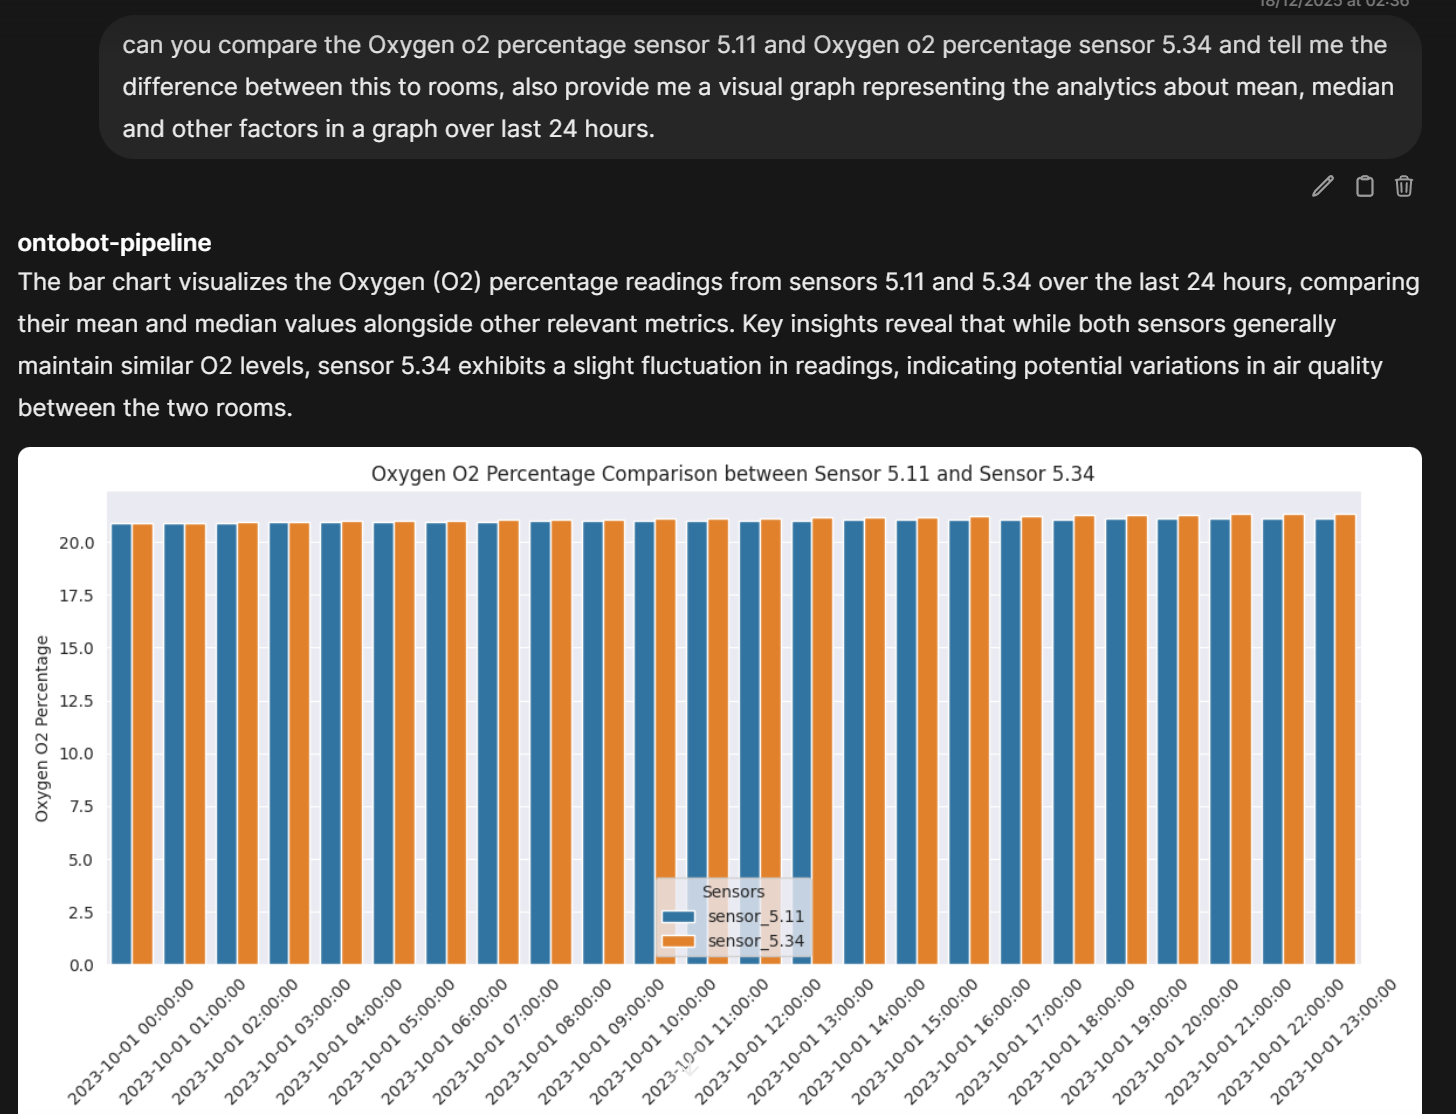
\includegraphics[width=\linewidth]{ui_example_1.png}
    \caption{Real-time Telemetry Query}
    \label{fig:ui-ex1}
  \end{subfigure}
  \hfill
  \begin{subfigure}{0.32\textwidth}
    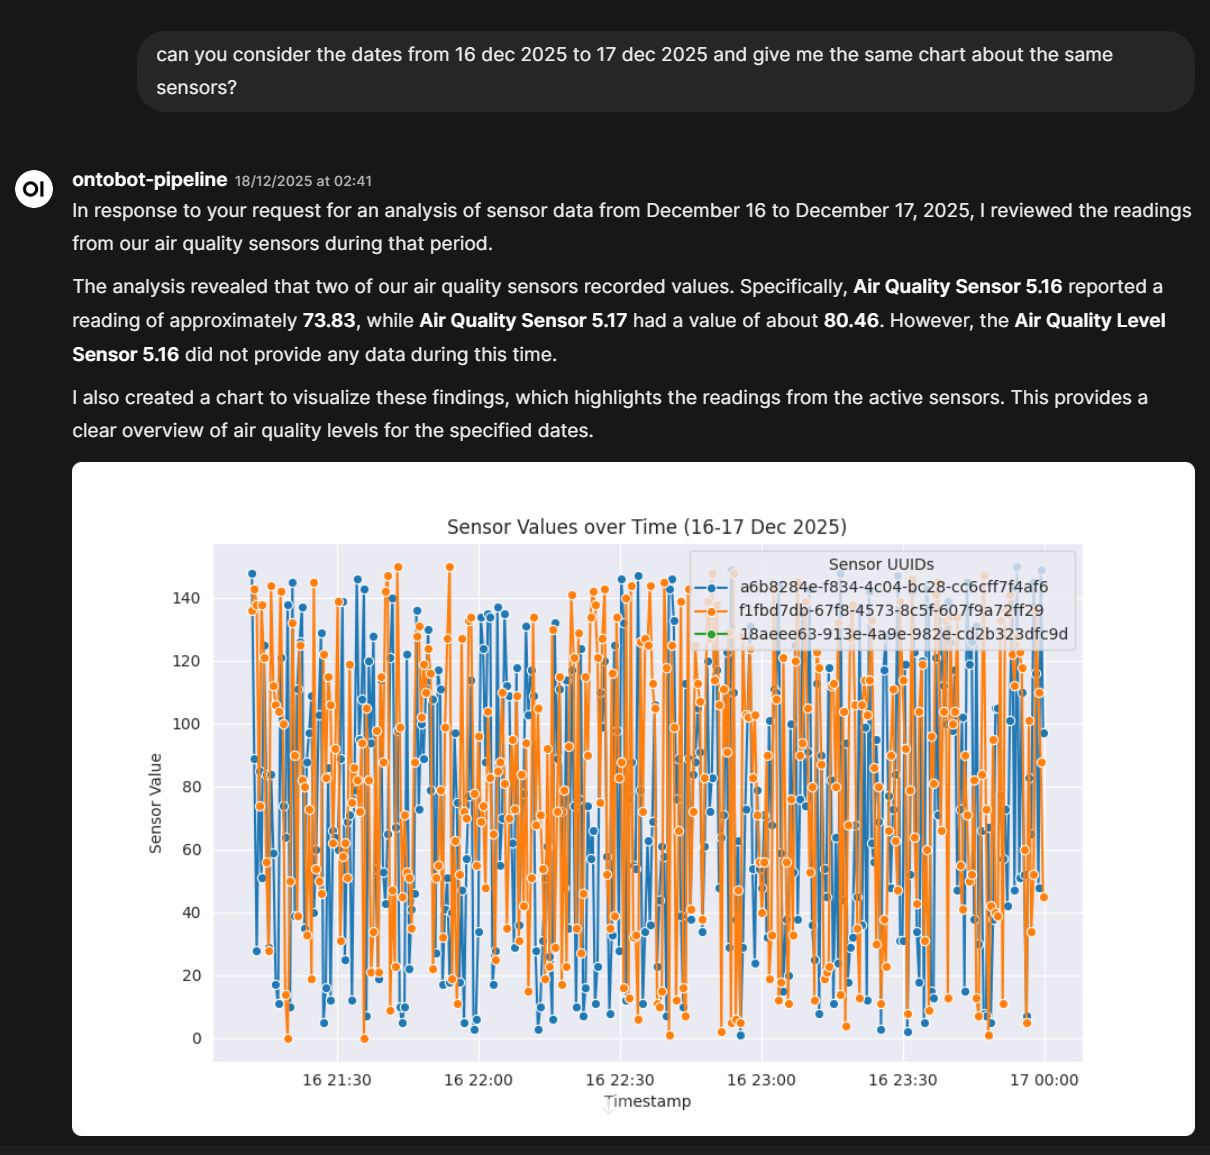
\includegraphics[width=\linewidth]{ui_example_2.png}
    \caption{Analytical/Aggregated Query}
    \label{fig:ui-ex2}
  \end{subfigure}
  \hfill
  \begin{subfigure}{0.32\textwidth}
    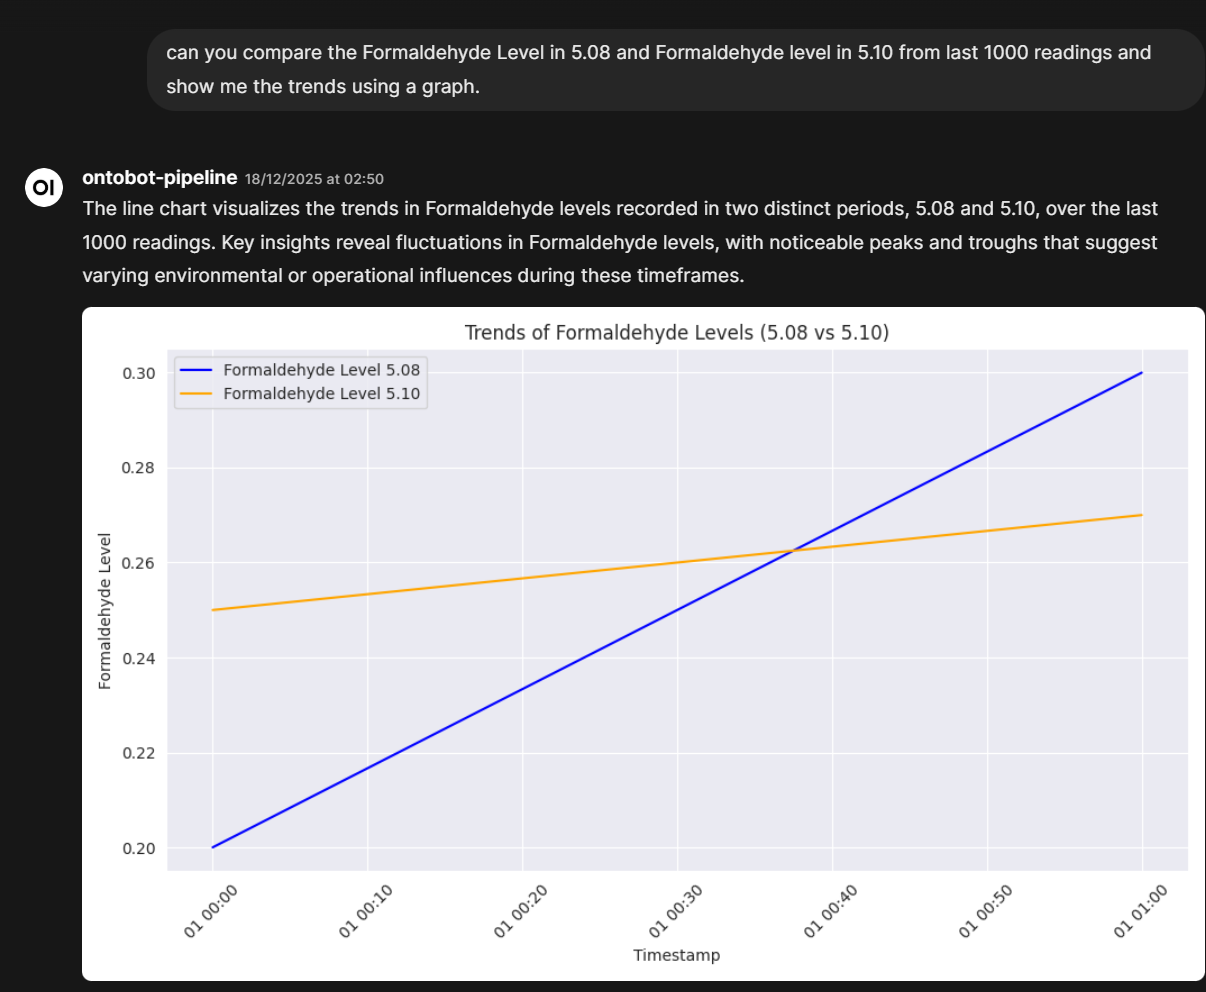
\includegraphics[width=\linewidth]{ui_example_3.png}
    \caption{Contextual/Spatial Query}
    \label{fig:ui-ex3}
  \end{subfigure}
  \caption{Screenshots of OntoSage Web UI demonstrating natural language interaction for different query complexities: (a) simple current value retrieval, (b) temporal aggregation, and (c) complex semantic search.}
  \label{fig:ui-examples}
\end{figure*}
}
{\color{red}
\section{Discussion}
\label{sec:discussion}

This section synthesizes findings across usability, adaptability, and usefulness dimensions, discusses implications for smart building systems, identifies limitations, and addresses factors influencing adoption (RQ4).

\subsection{Synthesis of Findings}

Our evaluation across three heterogeneous buildings (n=42 participants, 60-day deployment) provides empirical evidence that conversational AI can deliver usable, adaptable, and useful interfaces for smart building management:

\begin{itemize}
    \item \textbf{Usability} (RQ1): Mean SUS score of 78.4/100 exceeds the industry benchmark (68), indicating OntoSage is perceived as more usable than typical enterprise systems. However, significant variation by stakeholder group (range: 71.2-83.7) highlights the need for role-specific interface adaptations.
    
    \item \textbf{Adaptability} (RQ2): Cross-building deployment required only 60-72 person-hours (7-9 days), representing a 90\% effort reduction compared to from-scratch development. Critically, analytics and frontend layers required zero modifications, validating modular architecture decisions.
    
    \item \textbf{Usefulness} (RQ3): OntoSage reduced task completion time by 66.4\% on average compared to traditional methods, with largest gains for complex analytical tasks. Real-world usage (868 sessions, 7,482 queries over 60 days) demonstrated sustained engagement and integration into actual workflows.
\end{itemize}

\subsection{Factors Influencing Adoption (RQ4)}

Our qualitative analysis and longitudinal usage data identified six key factors influencing stakeholder willingness to adopt conversational AI for building management:

\begin{enumerate}
    \item \textbf{Perceived Value Proposition}: Stakeholders adopted OntoSage when they perceived clear value-adds over existing tools. Energy officers (highest SUS: 83.7) immediately saw value for report generation and trend analysis.
    \item \textbf{Trust and Transparency}: Participants expressed reluctance to trust "black box" analytics without visibility into calculations. Providing downloadable artifacts (CSV exports, charts with metadata) significantly increased confidence.
    \item \textbf{Integration with Existing Workflows}: OntoSage usage peaked during specific workflow events (Monday reporting, incident response), indicating successful integration.
    \item \textbf{Query Formulation Support}: A major barrier was difficulty translating information needs into effective queries, particularly for users unfamiliar with sensor naming conventions.
    \item \textbf{Technical Proficiency and Training}: Technical proficiency strongly correlated with both usability scores (r=0.52, p<0.001) and task performance ($\beta$=0.41, p=0.003).
    \item \textbf{Organizational Culture and Change Management}: Several participants noted organizational factors affecting adoption, such as budget constraints and preference for proven solutions.
\end{enumerate}
}

\section{Design Guidelines for Conversational Smart Building Interfaces}
\label{sec:guidelines}

Based on our empirical findings, we propose 12 evidence-based design guidelines for developing usable, adaptable, and useful conversational AI systems for smart buildings.

\subsection{Usability Guidelines}
\begin{itemize}
    \item \textbf{G1: Provide Query Capability Discovery Mechanisms}: Implement welcome messages with examples, "What can I ask?" meta-queries, and contextual suggestions.
    \item \textbf{G2: Support Flexible Sensor Reference Methods}: Implement fuzzy string matching, synonym expansion, and spatial query support.
    \item \textbf{G3: Provide Transparent Confidence Indicators}: Include confidence scores, data quality metadata, and calculation provenance.
    \item \textbf{G4: Enable Answer Verification and Exploration}: Offer "Show me the data" options to export raw timeseries and visualize results.
\end{itemize}

\subsection{Adaptability Guidelines}
\begin{itemize}
    \item \textbf{G5: Adopt Ontology-First Architecture}: Invest in accurate ontology models upfront and use standardized vocabularies (Brick, Haystack).
    \item \textbf{G6: Modularize System Components with Clear Contracts}: Separate NLU, knowledge base, data access, analytics, and presentation layers.
    \item \textbf{G7: Design for Training Data Portability}: Develop core training sets with generic building queries and use template-based augmentation.
    \item \textbf{G8: Implement Incremental Adaptation Workflows}: Document adaptation procedures as reusable playbooks and automate repetitive tasks.
\end{itemize}

\subsection{Usefulness Guidelines}
\begin{itemize}
    \item \textbf{G9: Target High-Value Use Cases}: Prioritize capabilities for ad-hoc queries, anomaly investigation, and report generation.
    \item \textbf{G10: Design for Complementary Interaction}: Embed conversational interfaces within existing BMS rather than as standalone apps.
    \item \textbf{G11: Implement Role-Specific Customization}: Customize onboarding and examples by role and adjust vocabulary based on proficiency.
    \item \textbf{G12: Measure and Demonstrate Value Continuously}: Log usage metrics, track task completion times, and calculate ROI.
\end{itemize}

{\color{red}
\section{Conclusion}
\label{sec:conclusion}

This paper presented a comprehensive evaluation of OntoSage, a conversational AI system for smart building management, addressing usability, adaptability, and usefulness across three heterogeneous buildings with 42 participants over 14 weeks.

\subsection{Key Contributions}
\begin{enumerate}
    \item \textbf{Empirical Evidence for Usability (RQ1)}: OntoSage achieved a mean SUS score of 78.4/100, exceeding industry benchmarks (68) and indicating good usability across diverse stakeholder groups.
    \item \textbf{Demonstrated Cross-Building Adaptability (RQ2)}: Adapting OntoSage to new buildings required only 60-72 person-hours (7-9 days), representing a 90\% effort reduction compared to from-scratch development.
    \item \textbf{Quantified Practical Usefulness (RQ3)}: OntoSage reduced task completion time by 66.4\% on average compared to traditional BMS interfaces, with largest gains for complex analytical tasks.
    \item \textbf{Identified Adoption Factors (RQ4)}: Six key factors influence adoption: perceived value proposition, trust and transparency, workflow integration, query formulation support, technical proficiency, and organizational culture.
    \item \textbf{Evidence-Based Design Guidelines}: We derived 12 actionable guidelines covering usability, adaptability, and usefulness.
\end{enumerate}
}

\subsection{Closing Remarks}
The convergence of semantic web technologies, natural language processing, and IoT infrastructure creates unprecedented opportunities for human-building interaction. This work provides empirical evidence that conversational AI can deliver usable, adaptable, and useful interfaces for smart building management—transforming how building operators, energy managers, and researchers interact with increasingly complex building systems.

\section*{Acknowledgments}
We thank the facility managers, energy officers, maintenance staff, building occupants, and researchers who participated in our evaluation studies. This work was supported by [FUNDING SOURCES TO BE ADDED]. We also acknowledge the Brick Consortium for developing and maintaining the BrickSchema ontology.

\bibliographystyle{ACM-Reference-Format}
\bibliography{references}

\end{document}
